\chapter{Solving $\textbf{Ax = b}$}
\section{Interpretations}

We aim to solve $\textbf{Ax} = \textbf{b}$ where $b \in \mathbb{C}^m$ and $\textbf{A} \in \mathbb{C}^{m\times n}$, and we want to determine if solution $\textbf{x}$ exists and whether it is unique. \\

Otherwise, if there is no solution, we pick the best approximation. We are also interested when $m\neq n $, when there is no solutions, or if they are not unique.\\

Estimating $\textbf{x}$ from $\textbf{Ax} = \textbf{b}$ is an inverse problem. An example in engineering: when the equations in $\textbf{A}$ models a distortion filter operation on some data, and we want to want restore $\textbf{x}$. An example of distortion could be motion blur in a photo, or room echo in a sound recording.\\

\begin{figure}[H]
    \centering
    
\includegraphics[width=0.7\linewidth]{img/conv_blur.png}
    
    
\end{figure}

\subsubsection*{Geometric Interpretation}
In the context of linear algebra, the equation \(Ax = b\) can be interpreted in both pure mathematical and geometrical terms as a system of linear equations. 

\begin{itemize}
    \item When \(m = n\), we have an equal number of equations and unknowns, which constitutes a square system. For instance, consider the system
    \[
    \begin{pmatrix}
    1 & 2 \\
    1 & -1 \\
    \end{pmatrix}
    \begin{pmatrix}
    x_1 \\
    x_2 \\
    \end{pmatrix}
    =
    \begin{pmatrix}
    4 \\
    1 \\
    \end{pmatrix},
    \]
    where each equation represents a line in a two-dimensional space. The intersection of two non-parallel lines signifies a unique solution.

    \item If the lines represented by the equations are parallel, the system may either have no solution or infinitely many solutions (the lines coincide). The \emph{rank} of matrix \(A\) is a critical determinant in identifying the uniqueness of the solution.

    \item In the case where \(m > n\), implying more equations than unknowns, the system is referred to as `tall'. Generally, such systems do not have a unique solution, as the equations may intersect at multiple points unless several of them overlap.

    \item Conversely, when \(m < n\), meaning there are more unknowns than equations, the system is described as `fat'. An example of this is when \(m = 2\) and \(n = 3\); we are dealing with two planes in a three-dimensional space. Unless the planes are parallel, they intersect along a line, leading to an infinite number of solutions. Thus, the solution, if it exists, is not unique.
\end{itemize}
\subsubsection*{Vector Space Interpretation}

Consider the matrix equation \( \mathbf{Ax} = \mathbf{b} \). This can be interpreted within the framework of vector spaces as follows:

\begin{itemize}
    \item The matrix \( \mathbf{A} \) can be seen as a linear transformation that maps vectors from \( \mathbb{C}^n \) to \( \mathbb{C}^m \).
    \item The operation \( \mathbf{Ax} \) corresponds to forming linear combinations of the columns of \( \mathbf{A} \), where the vector \( \mathbf{x} \) provides the combination coefficients.
    \item A solution to \( \mathbf{Ax} = \mathbf{b} \) is feasible if and only if the vector \( \mathbf{b} \) resides within the range (or column space) of \( \mathbf{A} \).
    \item The range space of \( \mathbf{A} \), denoted as \( \mathcal{R}(\mathbf{A}) \), contains all possible vectors \( \mathbf{b} \) that can be reached by the linear transformation \( \mathbf{A} \). If \( \mathcal{R}(\mathbf{A}) = \mathbb{C}^m \), meaning \( \mathbf{A} \) has full row rank, then any vector in \( \mathbb{C}^m \) can be obtained from \( \mathbf{A} \).
    \item {\color{green!55!blue}The existence of a solution is indicated by \( \mathbf{b} \) being in the range space of \( \mathbf{A} \), while the null space of \( \mathbf{A} \) determines the uniqueness. Specifically, if the null space of \( \mathbf{A} \) contains only the zero vector (is trivial), the solution to \( \mathbf{Ax} = \mathbf{b} \) is unique.}
    \item {\color{green!55!blue}Conversely, if the null space of \( \mathbf{A} \) is non-trivial, possessing vectors other than the zero vector, multiple solutions to \( \mathbf{Ax} = \mathbf{b} \) may exist.}
\end{itemize}


\section{Existence and Uniqueness}
The previous section is summarised by these theorems:

\begin{theorembox}{Existence}
Let $\textbf{A} \in \mathbb{C}^{m\times n}$.
\begin{enumerate}
    \item For each $\textbf{b} \in \mathbb{C}^m$ there exists at least one solution $\textbf{Ax}=\textbf{b}$
    \item The range space of \textbf{A} is full: $\mathcal{R}(\textbf{A}) = \mathbb{C}^m$
    \item $rank(\textbf{A}) = m$
    \item \textbf{A} is full row rank, so its rows are linearly independent.
These conditions imply $m\leq n$, a fat or square matrix.
\end{enumerate}
\end{theorembox}
\begin{theorembox}{Uniqueness}
Let $\textbf{A} \in \mathbb{C}^{m\times n}$.
\begin{enumerate}
    \item If there exists a solution to $\textbf{Ax}=\textbf{b}$,it is unique
    \item The null space of \textbf{A} is trivial (containing nothing but the zero vector)
    \item $rank(\textbf{A}) = n$
    \item \textbf{A} is full column rank, so its columns are linearly independent.
\end{enumerate}
These conditions imply $m\geq n$, a tall or square matrix.
\end{theorembox}

\begin{theorembox}{Existence and Uniqueness}
Let $\textbf{A} \in \mathbb{C}^{m\times n}$.
\begin{enumerate}
    \item For each $\textbf{b} \in \mathbb{C}^m$ there exists at least one solution $\textbf{Ax}=\textbf{b}$ and it is unique
    \item The range space of \textbf{A} is $m$: $\mathcal{R}(\textbf{A}) = \mathbb{C}^m$
    \item $rank(\textbf{A}) = m = n$ and \textbf{A}'s null space is trivial.
    \item \textbf{A} is square and nonsingular, so it has a determinant $\neq 0$
\end{enumerate}
\end{theorembox}

\begin{enumerate}
    \item Consider the matrix 
    \[
    A = \begin{pmatrix}
    4 & 8 & 6 \\
    0 & 4 & 7
    \end{pmatrix}.
    \]
    The rows are linearly independent, so for every vector \( \mathbf{b} \) in \( \mathbb{C}^2 \), there is at least one solution to \( A\mathbf{x} = \mathbf{b} \).

    \item The matrix
    \[
    A = \begin{pmatrix}
    1 & 0 & 1 \\
    0 & 1 & 1 \\
    1 & 1 & 2
    \end{pmatrix}
    \]
    has three rows but only rank 2. The conditions for the existence theorem are not satisfied, and there exist vectors \( \mathbf{b} \) for which \( A\mathbf{x} = \mathbf{b} \) has no solution. For example, \( \mathbf{b} = \begin{pmatrix} 0 & 0 & 1 \end{pmatrix}^\text{T} \).

    \item The matrix
    \[
    A = \begin{pmatrix}
    6 & 5 & 6 & 3 \\
    2 & 3 & 0 & 1 \\
    4 & 4 & 3 & 2
    \end{pmatrix}
    \]
    has more columns than rows and is not full row rank. Thus, the conditions for the existence theorem are not met, and a solution to \( A\mathbf{x} = \mathbf{b} \) does not always exist. Remember, having 'more unknowns than equations' or being 'underdetermined' does not guarantee the existence of a solution; having 'full row rank' does.
    \item Given the matrix 
\[ A = \begin{pmatrix} 0 & 1 \\ 1 & 1 \\ 1 & 0 \end{pmatrix}, \]
the columns are linearly independent. Therefore, for every vector \( \mathbf{b} \) in \( \mathbb{C}^2 \), there exists a unique solution to \( A\mathbf{x} = \mathbf{b} \). For example, if \( \mathbf{b} = \begin{pmatrix} 4 \\ 6 \\ 2 \end{pmatrix} \), the unique solution is \( \mathbf{x} = \begin{pmatrix} 2 \\ 4 \end{pmatrix} \). However, for \( \mathbf{b} = \begin{pmatrix} 1 \\ 0 \\ 0 \end{pmatrix} \), no solution exists.
    \item For the matrix 
\[ A = \begin{pmatrix} 1 & 0 & 1 \\ 0 & 1 & 1 \\ 1 & 1 & 2 \end{pmatrix}, \]
the columns are linearly dependent, with the null space being the span of \( \begin{pmatrix} 1 \\ 1 \\ -1 \end{pmatrix} \). Thus, neither uniqueness nor existence of the solution is guaranteed.
    \item Consider the matrix 
\[ A = \begin{pmatrix} 2 & 5 & 3 \\ 3 & 5 & 2 \\ 3 & 7 & 4 \\ 7 & 8 & 1 \end{pmatrix}. \]
The columns are linearly dependent, which means that even though the system is overdetermined, uniqueness of the solution cannot be assured.

\end{enumerate}

Our goal is to develop a single method that either finds \textbf{x} as the solution to $\textbf{Ax}=\textbf{b}$ if it exists, or find the best approximation.
\section{Four Fundamental Subspaces}
Given a linear mapping $A: \mathbb{C}^n \rightarrow \mathbb{C}^m$ represented by the matrix $A \in \mathbb{C}^{m \times n}$, we consider two important concepts: the range (or column space) of $A$, denoted as $\mathcal{R}(A)$, and the null space (or kernel) of $A$, denoted as $\mathcal{N}(A)$.

Exploring further, let us examine the adjoint of $A$, denoted as $A^H$, which maps vectors from $\mathbb{C}^m$ to $\mathbb{C}^n$. It is crucial to understand that $A^H$ is not necessarily the inverse of $A$ but rather the conjugate transpose of $A$.

The range of $A^H$, $\mathcal{R}(A^H)$, and the null space of $A^H$, $\mathcal{N}(A^H)$, can be defined analogously. These subspaces interact with each other in the following ways, which we state without proof:

\begin{itemize}
  \item $\mathbb{C}^m = \mathcal{R}(A) \oplus \mathcal{N}(A^H)$, where $\oplus$ denotes the direct sum, and $\mathcal{R}^\perp(A) = \mathcal{N}(A^H)$, meaning the orthogonal complement of the range of $A$ is the null space of $A^H$.
  \item $\mathbb{C}^n = \mathcal{R}(A^H) \oplus \mathcal{N}(A)$, and $\mathcal{R}^\perp(A^H) = \mathcal{N}(A)$, indicating that the orthogonal complement of the range of $A^H$ is the null space of $A$.
\end{itemize}


\begin{figure}[H]
    \centering
    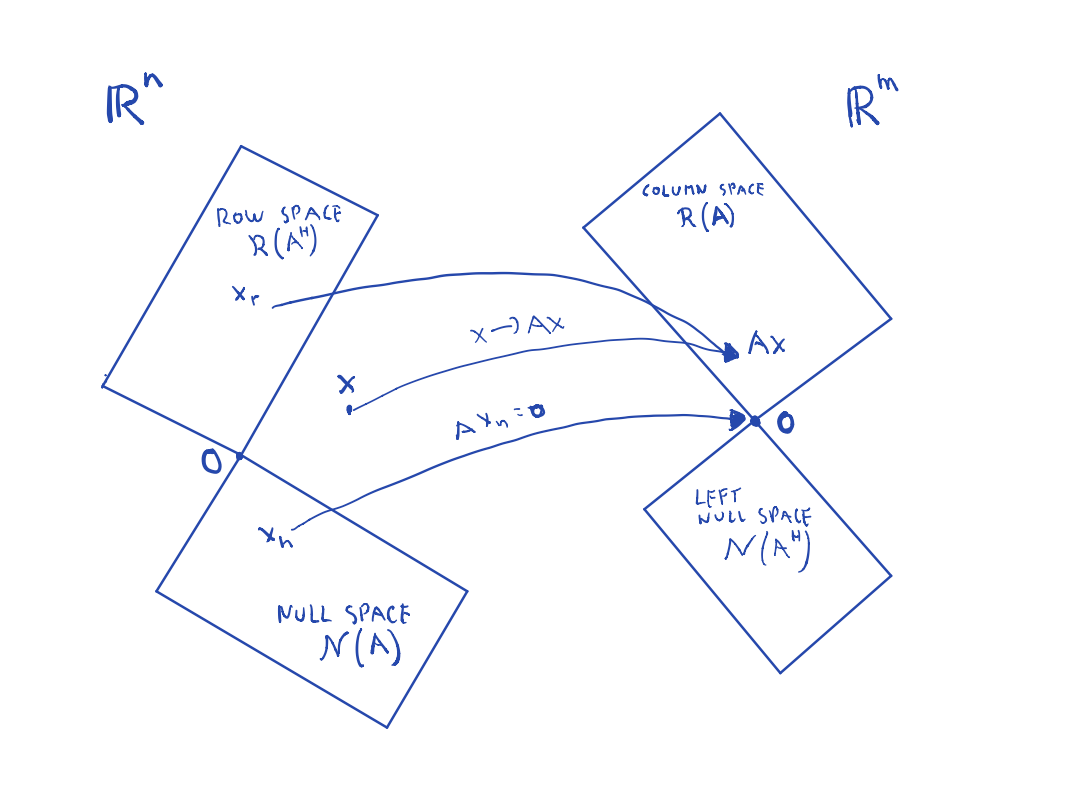
\includegraphics[width=0.75\linewidth]{img/subspaces.png}
    \caption{Visual representation of the four fundamental subspaces in linear algebra. The null space and row space are mapped through $A$ and $A^H$ to the column space and left null space respectively. Each vector in the null space maps to the zero vector in the column space, while vectors in the row space and beyond map into the column space. Would be nice to replace this with an actual diagram, will do this when I have more time}
\end{figure}

\begin{examplebox}{Sample subspaces question}
    Consider the matrix 
\[
A = \begin{pmatrix}
1 & 1 & 1 \\
0 & 1 & 0 \\
0 & 0 & 0 \\
\end{pmatrix}.
\]
Our goal is to find the four fundamental subspaces of $A$: the column space $\mathcal{R}(A)$, the null space $\mathcal{N}(A)$, the row space $\mathcal{R}(A^H)$, and the left null space $\mathcal{N}(A^H)$.

\subsubsection*{Column Space and Null Space}
Since $A$ is already in row-echelon form, the range space (or column space) of $A$ is spanned by the first two columns of $A$:
\[
\mathcal{R}(A) = \text{span}\left\{ \begin{pmatrix} 1 \\ 0 \\ 0 \end{pmatrix}, \begin{pmatrix} 1 \\ 1 \\ 0 \end{pmatrix} \right\}.
\]
The dimension of the null space of $A$ is given by the Rank-Nullity Theorem:
\[
\dim(\mathcal{N}(A)) = 3 - \text{rank}(A) = 1.
\]
A basis for the null space, found by solving $A\bm{n} = \bm{0}$, is:
\[
\mathcal{N}(A) = \text{span}\left\{ \begin{pmatrix} 1 \\ 0 \\ -1 \end{pmatrix} \right\}.\]

\subsubsection*{Row Space and Left Null Space}
The row space of $A^H$, which is the column space of $A$, has already been determined. The left null space is the orthogonal complement of the row space in $\mathbb{C}^m$:
\[
\mathcal{N}(A^H) = \text{span}\left\{ \begin{pmatrix} 0 \\ 0 \\ 1 \end{pmatrix} \right\}.
\]
Finally, the row space of $A$ (which is the column space of $A^H$) can be obtained by taking the non-zero rows of $A$:
\[
\mathcal{R}(A^H) = \text{span}\left\{ \begin{pmatrix} 1 \\ 1 \\ 1 \end{pmatrix}, \begin{pmatrix} 0 \\ 1 \\ 0 \end{pmatrix} \right\}.
\]
\end{examplebox}


 \section{Inverses}
 We classify inverses of matrices based on their dimensions and rank:

\begin{itemize}
    \item A square and nonsingular (invertible) matrix $A$ possesses an inverse $A^{-1}$ such that $AA^{-1} = A^{-1}A = I$, where $I$ is the identity matrix.
    \item Non-square matrices do not have an inverse in the traditional sense; however, they may have a left or right inverse under certain conditions:
    \begin{itemize}
        \item A \textbf{left inverse} of a matrix $A$ exists if there is a matrix $B$ such that $BA = I$ (and typically $AB \neq I$), which requires $A$ to be full column rank.
        \item A \textbf{right inverse} of a matrix $A$ exists if there is a matrix $C$ such that $AC = I$, necessitating $A$ to be full row rank.
    \end{itemize}
    \item It is important to note that these inverses may not be unique.
\end{itemize}


 
\section{Projections and Approximations}
\begin{theorembox}{Projection Theorem}
Let \( V \) be a closed subspace of Hilbert space \( H \) and let \( x \) be a vector in \( H \).
\begin{enumerate}
  \item \textbf{Existence:} There exists \( \hat{x} \in V \) such that \( \|x - \hat{x}\| \leq \|x - v\| \) for all \( v \in V \).
  \item \textbf{Orthogonality:} \( x - \hat{x} \perp V \) is necessary and sufficient for determining \( \hat{x} \).
  \item \textbf{Uniqueness:} The vector \( \hat{x} \) is unique.
  \item \textbf{Linearity:} \( \hat{x} = Px \) where \( P \) is a linear operator that depends on \( V \) and not on \( x \).
  \item \textbf{Idempotency:} \( P(Px) = Px \) for all \( x \in H \).
  \item \textbf{Self-adjointness:} \( P = P^H \).
\end{enumerate}
\end{theorembox}

\begin{definitionbox}{Projection Matrix}
    Given a matrix \( A \) and a vector \( \mathbf{b} \), we seek to project \( \mathbf{b} \) onto the column space of \( A \). The projection is denoted by \( A\mathbf{x} \), where \( \mathbf{x} \) is the vector in the column space of \( A \) that is closest to \( \mathbf{b} \).

\subsection*{Orthogonality Principle}
The difference \( \mathbf{b} - A\mathbf{x} \) is orthogonal to the column space of \( A \), implying that it lies in the null space of \( A^T \). Hence, we have:
\begin{equation}
    A^T(\mathbf{b} - A\mathbf{x}) = 0
\end{equation}

\subsection*{Derivation}
Rearranging the above equation, we obtain:
\begin{align}
    A^T\mathbf{b} &= A^TA\mathbf{x} \\
    \Rightarrow \mathbf{x} &= (A^TA)^{-1}A^T\mathbf{b}
\end{align}
This equation provides us with the least squares solution for \( \mathbf{x} \).

\subsection*{Projection Matrix}
The matrix that projects any vector \( \mathbf{b} \) onto the column space of \( A \) is known as the projection matrix, \( P \), and is given by:
\begin{equation}
    P = A(A^TA)^{-1}A^T
\end{equation}
This projection matrix has the property that \( P\mathbf{b} = A\mathbf{x} \), which is the projection of \( \mathbf{b} \) onto the column space of \( A \).

\begin{figure}[H]
    \centering
\begin{tikzpicture}[scale=0.8, >=Stealth]
    \begin{axis}[
        axis lines=middle,
        xmin=-1, xmax=3,
        ymin=-1, ymax=3,
        xlabel={$x$},
        ylabel={$y$},
        xtick={0}, ytick={0},
        xticklabels={,,}, yticklabels={,,}
    ]

    % Line A passing through the origin
    \addplot[domain=-1:3, samples=2, green, thick] {0.5*x};
    \node[label={0:{\(A\)}}, inner sep=0pt] at (axis cs:2.3,1.1) {};

    % Vector b
    \draw[red, thick, -{>[length=3mm]}] (0,0) -- (2,3) node[midway, above left] {\(\mathbf{b}\)};

    % Projection of b onto A (Ax)
    \draw[orange, thick, -{>[length=3mm]}] (0,0) -- (2,1) node[midway, below] {\(A\mathbf{x}\)};

    % Error vector b - Ax
    \draw[black, dashed, thick, -{>[length=3mm]}] (2,1) -- (2,3) node[midway, right] {\(\mathbf{b} - A\mathbf{x}\)};

    \end{axis}
\end{tikzpicture}
\end{figure}
 
\end{definitionbox}
\section{Gram-Schmidt Orthogonalisation Process}


The Gram-Schmidt process is a method for orthonormalising a set of vectors in an inner product space. It is a direct application of the projection theorem, and it helps to form an orthonormal basis, which is a cornerstone in linear algebra and has crucial applications in signal processing and systems theory.

\subsection*{Orthogonal and Orthonormal Matrices}

At the outset of our course, we discussed orthogonal matrices. Now, we delve into a practical use-case of these concepts.

\begin{itemize}
    \item An \textbf{orthogonal matrix} $A$ is a square matrix with real entries whose columns and rows are orthonormal vectors. That is, the transpose of $A$ is also its inverse: $A^\mathsf{T}A = AA^\mathsf{T} = I$, where $I$ is the identity matrix. 
    \item When we construct a matrix $A$ from a set of vectors $\{v_i\}_{i=1}^n$ that form an orthonormal basis, it satisfies this property. 
    \item Mathematically, if $v_i$ for $i = 1, 2, \ldots, n$ are orthonormal, then:
    \begin{equation}
        A = \begin{pmatrix}
            v_{1,1} & \cdots & v_{1,n} \\
            \vdots & \ddots & \vdots \\
            v_{n,1} & \cdots & v_{n,n}
        \end{pmatrix}
    \end{equation}
    \item Such matrices not only preserve lengths (due to maintaining the induced norm) but also angles between vectors when used in linear transformations.
\end{itemize}

\subsection*{The Process}

The essence of the Gram-Schmidt process is to take a set of linearly independent vectors and orthogonalise them while maintaining their span.

\begin{itemize}
    \item Start with any set of independent vectors $\{a, b, c\}$.
    \item First normalise vector $a$ to find $q_1$:
    \begin{equation}
        q_1 = \frac{a}{\|a\|}
    \end{equation}
    \item To find $q_2$, orthogonal to $q_1$, project $b$ onto $q_1$ and subtract this projection from $b$, then normalise:
    \begin{equation}
        q_2 = \frac{b - \text{proj}_{q_1}(b)}{\|b - \text{proj}_{q_1}(b)\|}
    \end{equation}
    \item The projection operator $P$ onto $q_1$ is defined as:
    
    \begin{equation}
        P = \frac{a a^\mathsf{T}}{a^\mathsf{T}a}
    \end{equation}
    \item For vector $c$, ensure it is orthogonal to both $q_1$ and $q_2$:
    \begin{equation}
        q_3 = \frac{c - \text{proj}_{q_1}(c) - \text{proj}_{q_2}(c)}{\|c - \text{proj}_{q_1}(c) - \text{proj}_{q_2}(c)\|}
    \end{equation}
    \item This process can be continued for higher dimensions. If there were a fourth vector $d$, we would subtract its projections onto $q_1$, $q_2$, and $q_3$ before normalizing.
\end{itemize}

\subsection*{Visualising the Concept}

Consider vectors $a$, $b$, and $c$ in a three-dimensional space. By applying the Gram-Schmidt process, we are essentially rotating and stretching the axes of our coordinate system such that each vector $q_i$ lies along one of these new axes, ensuring orthogonality and normality.

\begin{itemize}
    \item Visual representation of transforming vector $b$:
    \begin{equation}
        B = b - \frac{a a^\mathsf{T}}{a^\mathsf{T}a}b
    \end{equation}
    \item This transformed vector $B$ is now orthogonal to $a$.
    \item We then apply a similar approach to vector $c$ to ensure it is orthogonal to both $a$ and $B$:
    \begin{equation}
        C = c - \frac{a a^\mathsf{T}}{a^\mathsf{T}a}c - \frac{b b^\mathsf{T}}{b^\mathsf{T}b}c
    \end{equation}
\end{itemize}
Make sure to normalise the vectors after their transformations!\\
\textbf{In general we subtract from every new vector its projections in the directions already set.} Then we make the resulting vectors orthonormal, by dividing the vectors with their magnitudes.

\subsection*{Remarks}

The Gram-Schmidt process is an elegant way of generating an orthogonal set from a linearly independent set. It plays a significant role in many areas of mathematics and engineering, including the understanding of Fourier series, signal processing, and the method of least squares in statistics.

\section{Solutions, either exact or approximate}
% We take the derivative and set it to zero.\\


Let's consider the problem of finding a vector \( \mathbf{x} \) such that \( A\mathbf{x} = \mathbf{b} \), with a particular focus on matrices \( A \) that have full column rank.

\begin{itemize}
    \item A matrix \( A \) with full column rank is tall, implying that the columns of \( A \) are linearly independent. If a solution to the system \( A\mathbf{x} = \mathbf{b} \) exists, this solution is unique due to the full column rank of \( A \).
    
    \item To solve the system, we aim to find the left inverse of \( A \). This is because the left inverse allows us to compute the solution directly for a full column rank matrix.
    
    \item The solution process involves a somewhat convoluted but geometrically inspired approach. We seek a vector \( \mathbf{x}_{LS} \) that minimizes the norm \( \|A\mathbf{x}_{LS} - \mathbf{b}\| \), making it the least squares solution. This means that \( \|A\mathbf{x}_{LS} - \mathbf{b}\| \leq \|A\mathbf{x} - \mathbf{b}\| \) for any vector \( \mathbf{x} \).
    
    \item Consequently, if a solution to \( A\mathbf{x} = \mathbf{b} \) exists, then \( \mathbf{x}_{LS} \) is that solution, and it can be found by projecting \( \mathbf{b} \) onto the column space of \( A \).
\end{itemize}


\textbf{Claim:}

The vector $\widehat{x}$ minimises $||Ax-b||$ iff $A^H A\widehat{x} = A^Hb$, which is the normal equation.\\


\textbf{Proof:}
\begin{itemize}
    \item Minimizing $\|Ax - b\|$ is equivalent to minimizing $\|\hat{b} - b\|$ where $\hat{b} \in \mathcal{R}(A)$.
    \item By the projection theorem: $b - \hat{b} \in \mathcal{R}(A)^\perp \Rightarrow b - \hat{b} \in \mathcal{N}(A^H)$.
    \item Therefore, $A^H(b - \hat{b}) = 0 \Rightarrow A^Hb = A^H\hat{b} \Rightarrow A^HA\hat{x} = A^Hb$.
    \item Conversely $A^HA\hat{x} = A^Hb \Rightarrow A^H(b - A\hat{x}) = 0$.
\end{itemize}
\begin{figure}
    \centering
    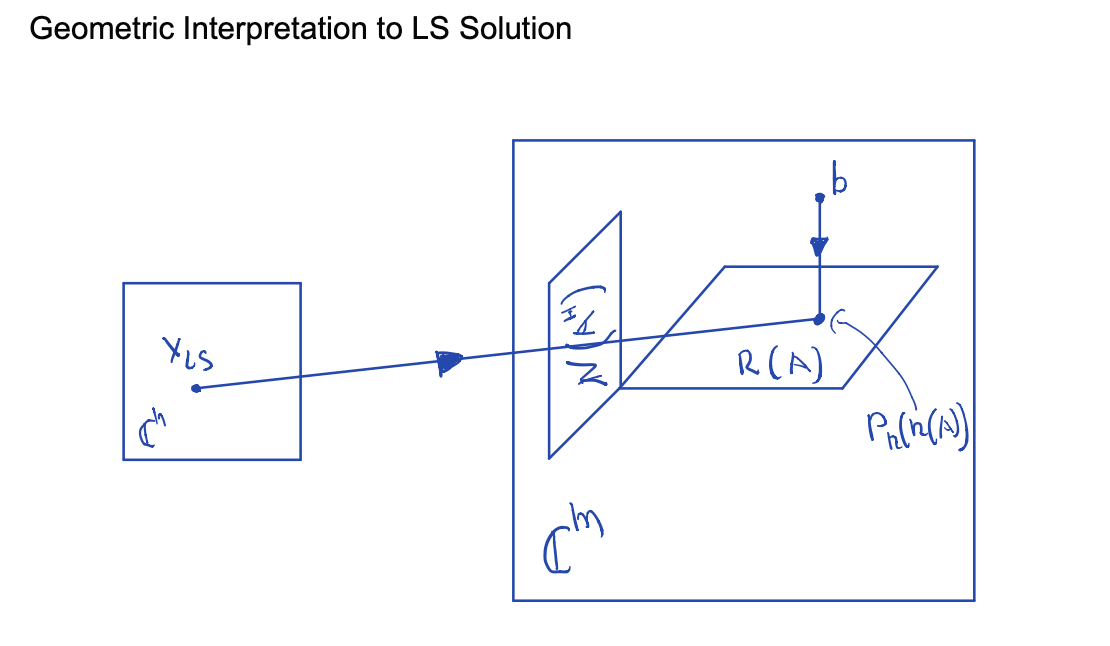
\includegraphics[width=0.75\linewidth]{img/geom_ls.png}
    
    
\end{figure}

% \begin{examplebox}{Title}
%     \begin{align*}
%     ||Ax = b|| \Rightarrow \\
%     \left| \left| \begin{pmatrix}
%         a_{11} & a_{12} \\
%         a_{21} & a_{22} \\
%     \end{pmatrix}
%     \begin{pmatrix}
%         x_1 \\ x_2
%     \end{pmatrix} =
%     \begin{pmatrix}
%         b_1 \\ b_2
%     \end{pmatrix}\right| \right| 
%     \end{align*}
% \end{examplebox}
\subsection{Example: Least-Square Deconvolution}
Assume you have a system that blurs an image, this is your FIR (finite impulse response) filter. You want to recover the original sharp image. However, this observed image is noisy. Using the deconvolution process, you would attempt to reverse the blurring to approximate the original image as closely as possible.\\

Given the output $\textbf{y}\in \mathbb{C}^{n+k-1}$ of the filter and the filter is represented by matrix $\textbf{A} \in \mathbb{C}^{(n+k-1)\times n}$, which is the convolution (Toeplitz) matrix associated with K-tap filter $\textbf{h}$. Each row of the Toeplitz matrix is a shifted version of the filter coeffficients (or taps).\\

If $\textbf{y}$ is noise-free, we can find the signal easily, but it is usually noisy. So we have the measured signal $\textbf{b} = \textbf{y}+\textbf{n}$ \\

We can solve for $\textbf{A}^H \textbf{A}\hat{\textbf{x}} = \textbf{A}^H\textbf{b}$, to get $\hat{\textbf{x}}$ that is the closest to the true signal \textbf{x}.

\begin{figure}[H]
    \centering
    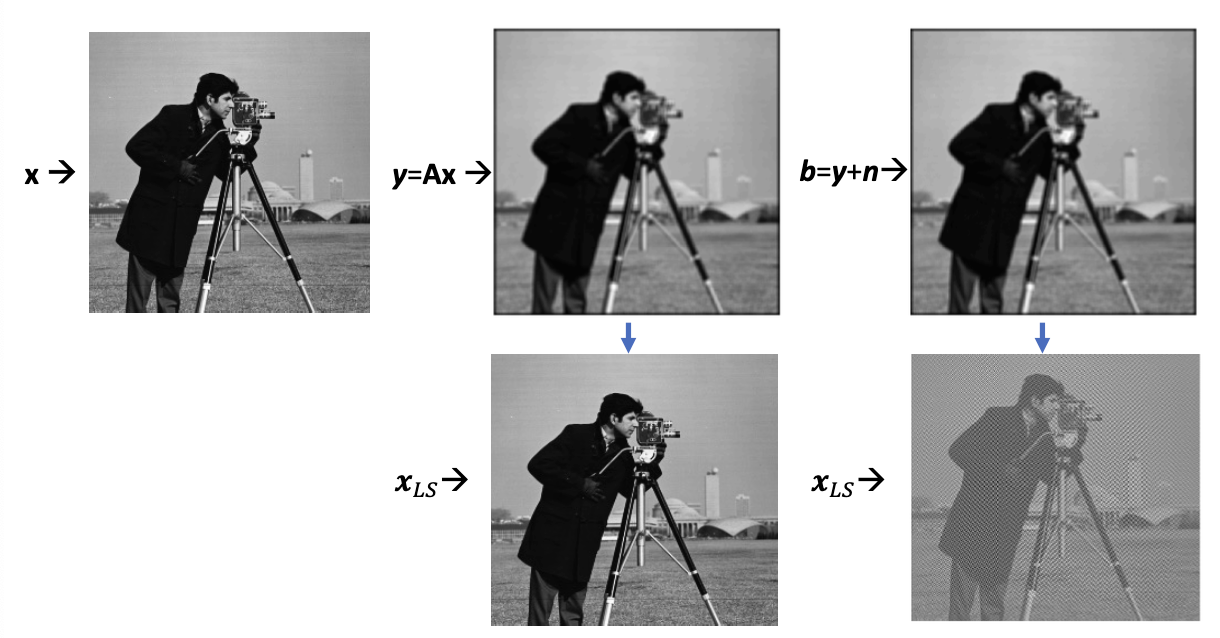
\includegraphics[width=0.75\linewidth]{img/ls-deconv.png}
    \caption{Some noise does end up back in the Least-Squares solution.}
    
\end{figure}
\begin{figure}[H]
    \centering
    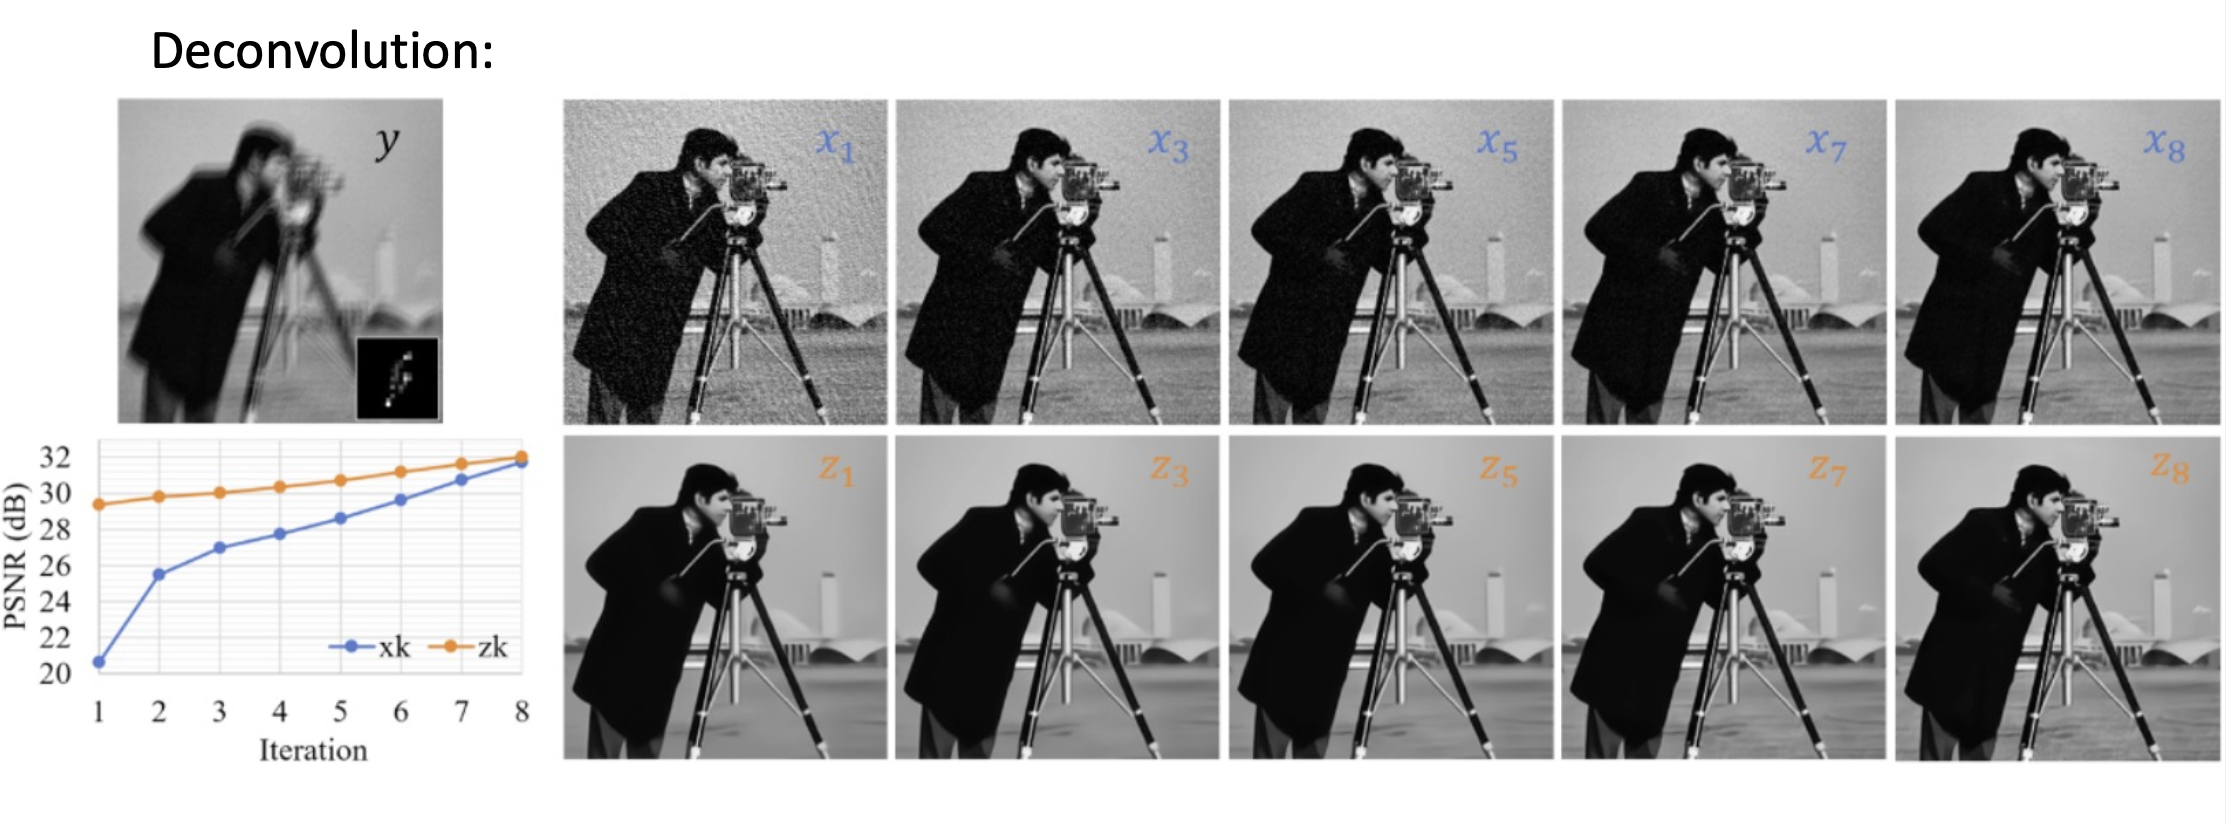
\includegraphics[width=1\linewidth]{img/deconv2.png}
    \caption{Enter Caption}
\end{figure}
\subsection{Example: High-Order Regression}
\textit{(Incomplete)}
% \subsection{Example: Least-Square Deconvolution}
\subsection{Solution (Full Row-Rank Case)}
\begin{itemize}
    \item We now understand how to find an approximate solution \(\textbf{Ax = b}\) in the full column rank case where a solution might exist.
    \item We now consider the full row rank case where \(\textbf{A}\) is fat and we know at least one solution exists.
    \item When the solution exists but is not unique, the set of all solutions has a special structure.
    \item Let \(\textbf{x}_p\) be a solution to \(\textbf{Ax}\textbf{b}\). Then any other solution is \[
    \textbf{x} = \textbf{x}_p
 + \textbf{z}\]
 where \(\textbf{z} \in \mathcal{N}(\textbf{A})    \).
    \item Then the solution to \(\textbf{Ax = b}\) is \(S = \{\textbf{x}_p\} + \mathcal{N}(\textbf{A})\) where \(S\) is a translated subspace of \(\mathcal{N}(\textbf{A)}\) also known as an \textbf{affine subspace}.
    \item We want to pick one of the infinitely many solutions – we look for the \textbf{minimum norm solution}: 
    \[ \min_{||\textbf{x}||} \textbf{Ax} = \textbf{b}\]
\end{itemize}

% \begin{examplebox}{Minimum Norm Solution Example}
%     \begin{itemize}
%         \item Let $\textbf{A} = [1,1]$  and suppose $\textbf{b} = 3$.
%         \item The set of all possible real solutions to $\textbf{Ax} = \textbf{b}$ is defined as $T = \{\textbf{x} : x_1 + x_2 =3  \}$ 
%         \item So $\textbf{x} = \begin{pmatrix}
%             \alpha \\ 3-\alpha 
%         \end{pmatrix} $ and $||x||^2 = \alpha ^2 + (3-\alpha^2)$
%         \item Taking the derivative of the norm and setting it to zero, we find the minimum norm solution \textbf{x}: \[\textbf{x} = \begin{pmatrix}
%             3/2 \\ 3/2
%         \end{pmatrix}\]
%     \end{itemize}



% \centering
% \begin{tikzpicture}[scale=1]
% % Coordinate system
% \draw[thick,->] (-3,0) -- (5,0) node[anchor=south] {$x_1$};
% \draw[thick,->] (0,-3) -- (0,5) node[anchor=west] {$x_2$};

% % Lines with arrows on both ends
% \draw[blue, thick, <->] (-2,-2) -- (3,3) node[anchor=south west] {$\mathcal{N}(A)^\perp$};
% \draw[blue, thick, <->] (-2,2) -- (2,-2) node[anchor=south east] {$\mathcal{N}(A)$};

% % Additional diagonal line
% \draw[blue, thick, <->] (3,-2) -- (-2,3) node[anchor=north] {};

% % Points and labels for the minimum norm solution
% \node[label={[label distance=0.5em]45:{$x_{MN}$}},circle,fill,inner sep=2pt] at (0.5,0.5) {};
% \node[anchor=south west] at (1,0.5) {$\left(\frac{3}{2},\frac{3}{2}\right)$};

% % Annotations
% \node[anchor=north, align=center] at (2.5,-2.5) {$S = \{ x \in \mathbb{R}^2 :$\\$ x_1 + x_2 = 3 \}$};
% \node[anchor=south, align=center] at (-2.5,2.5) {$\mathcal{N}(A) = \{ x \in \mathbb{R}^2 :$\\$ x_1 + x_2 = 0 \}$};

% \end{tikzpicture}




% \end{examplebox}

\begin{theorembox}{Dual Projection Theorem (without proof)}
Let \( T = \{x_p\} + S \) be an affine subspace of \( \mathbb{C}^n \). \\

Then the element \( t_{MN} \) of \( T \) with minimum norm exists, is unique, and satisfies \( t_{MN} \in T \cap S^{\perp} \).\\

Moreover, \( t_{MN} = P_{S^{\perp}}t \).\\

First, observe that the affine subspace \( T \) can be expressed as a translation of the subspace \( S \) by the vector \( x_p \). This translation does not affect the property of orthogonality, so the orthogonal complement of \( S \) is the same as the orthogonal complement of \( T \).\\

The existence and uniqueness of \( t_{MN} \) follow from the properties of Hilbert spaces. Specifically, since \( \mathbb{C}^n \) with the standard inner product is a Hilbert space, there exists a unique element of minimal norm in the closure of the convex set \( T \). The element \( t_{MN} \) is the projection of the origin onto the convex set \( T \), which exists and is unique due to the Hilbert space projection theorem.\\

To show that \( t_{MN} \in T \cap S^{\perp} \), we use the fact that for any \( t \in T \), the difference \( t - t_{MN} \) is orthogonal to \( S^{\perp} \) because the projection onto a closed convex set is the nearest point in the set to the origin, and all other points in \( T \) must be further away.\\

Finally, \( t_{MN} = P_{S^{\perp}}t \) because the projection operator \( P_{S^{\perp}} \) is idempotent and self-adjoint, meaning that \( P_{S^{\perp}} \) applied to any \( t \in T \) yields the unique closest point in \( T \cap S^{\perp} \), which is \( t_{MN} \).\\

Therefore, \( t_{MN} \) is the minimum norm element of \( T \), it is unique, and it lies in both \( T \) and \( S^{\perp} \).
\\
\end{theorembox}

\begin{theorembox}{Minimum Norm Theorem}
Let \( \textbf{Ax} = \textbf{b} \) and let \( A \) be a full-row rank matrix.\\
Amongst all the \( x \in \mathbb{C}^n \) satisfying \( \textbf{Ax} = \textbf{b} \), there exists a unique solution with minimum norm. It lies in \( \mathcal{R}(A^H) \) and is given by \( \textbf{x}_{MN} = \textbf{A}_{MN}b \) with \( \textbf{A}_{MN} = \textbf{A}^\textbf{H}(\textbf{AA}^\textbf{H})^{-1} \).\\

If \( \textbf{x}_p \) is a solution to \( \textbf{Ax} = \textbf{b} \) then all the solutions are in the affine subspace \( T = \{\textbf{x}_p\} + \mathcal{N}(A) \). \\

Using the Dual Projection Theorem we conclude that \[ x_{MN} \in T \cap \mathcal{N}(A)^{\perp} = T \cap \mathcal{R}(A^H) \] \\

Since \( x_{MN} \in \mathcal{R}(A^H) \) implies \( x_{MN} = A^Hz \) and hence \( b = Ax_{MN} = (AA^H)z \).\\

Therefore, \( z = (AA^H)^{-1}b \) which implies that \( x_{MN} = A^H(AA^H)^{-1}b \).
\end{theorembox}

\section{Computing Left and Right Inverses}
\subsubsection*{Claim:}
Assume $\textbf{A}$ is tall, full-column rank, then $\textbf{A}$ has a left inverse $\textbf{A}_{left}$

\subsubsection*{Sketch of Proof:}
$\textbf{A}^\top \textbf{A}$ is full rank, so $(\textbf{A}^\top \textbf{A})^{-1}$ exists. Then $\textbf{A}_{left} = (\textbf{A}^\top \textbf{A})^{-1} \textbf{A}^\top$ 

\subsubsection*{Likewise:}
Assume $\textbf{A}$ is fat and full-row rank, then \textbf{A} has right invese $\textbf{A}_{right}$ and $\textbf{A}_{right} = \textbf{A}^\top (\textbf{AA}^\top)^{-1}$

\section{Least-Square Problems with Linear Constraints}
Revisiting the minimum norm solution approach – we recall that in the full row-rank case, at least one solution exists. Since there are infinitely many solutions, we look for a specific one:

\[\min||x||^2 \text{subject to } \textbf{Ax}=\textbf{b}\]

We can interpret the equation above differently as a least-squares minimisation with linear constraints.

\[x=\begin{pmatrix}
    x_1\\x_2\\ \vdots \\ x_n
\end{pmatrix}
b=\begin{pmatrix}
    b_1\\b_2\\ \vdots \\ b_n
\end{pmatrix}
\]

% (what diagram did he use in the slide????)

\[\min||\textbf{y}-\textbf{Cx}||^2 \text{subject to } \textbf{Ax}=\textbf{b}\]

To solve this constrained optimisation problem, we introduce the method of Lagrangian multipliers. The Lagrangian function is given by:
\[
L(\mathbf{x}, \boldsymbol{\lambda}) = \|\mathbf{y} - \mathbf{C}\mathbf{x}\|^2 + \sum_{i=1}^{m} \lambda_i (\mathbf{a}_i^\mathsf{T}\mathbf{x} - b_i),
\]
where $\mathbf{a}_i^\mathsf{T}$ are the rows of $\mathbf{A}$ and $\lambda_i$ are the Lagrangian multipliers associated with each constraint.

\[
L(\mathbf{x}, \boldsymbol{\lambda}) = (\mathbf{y} - \mathbf{C}\mathbf{x})^\mathsf{T}(\mathbf{y} - \mathbf{C}\mathbf{x}) + \boldsymbol{\lambda}^\mathsf{T}\mathbf{A}\mathbf{x} - \boldsymbol{\lambda}^\mathsf{T}\mathbf{b}.
\]


To find the minimum, we take the gradient of the Lagrangian with respect to $\mathbf{x}$ and set it to zero:
\[
\frac{\partial L(\mathbf{x}, \boldsymbol{\lambda})}{\partial \mathbf{x}} = 0 \implies 2\mathbf{C}^\mathsf{T}\mathbf{C}\mathbf{x} - 2\mathbf{C}^\mathsf{T}\mathbf{y} + \mathbf{A}^\mathsf{T}\boldsymbol{\lambda}=\mathbf{0}.
\]

By combining this set of linear equations with the feasibility conditions $\mathbf{A}\mathbf{x} = \mathbf{b}$, we can write the optimality conditions as one set of $m+n$ linear equations in the variables $(\mathbf{x}; \boldsymbol{\lambda})$:
\[
\begin{pmatrix}
2\mathbf{C}^\mathsf{T}\mathbf{C} & \mathbf{A}^\mathsf{T} \\
\mathbf{A} & \mathbf{0}
\end{pmatrix}
\begin{pmatrix}
\mathbf{x} \\
\boldsymbol{\lambda}
\end{pmatrix}
=
\begin{pmatrix}
2\mathbf{C}^\mathsf{T}\mathbf{y} \\
\mathbf{b}
\end{pmatrix}.
\]

Solving this system yields the vector $\mathbf{x}$ that minimises the squared norm while satisfying the constraints.\\

Note that the square matrix $\begin{pmatrix}
2\mathbf{C}^\mathsf{T}\mathbf{C} & \mathbf{A}^\mathsf{T} \\
\mathbf{A} & \mathbf{0}
\end{pmatrix}
\begin{pmatrix}
\mathbf{x} \\
\boldsymbol{\lambda}
\end{pmatrix}$ is invertible iff \textbf{A} is full row rank and $\begin{pmatrix}
    \textbf{C}\\ \textbf{A} 
\end{pmatrix}$ is full column-rank.






